\section{Evidence, submission ledger and requirement coverage}
\label{app:ledger}
The evidence used here has three levels. The results document supplies screenshots of submission IDs,
filenames, status and displayed scores, plus a rank beside each phase heading. Executed outputs in the
later notebooks supply local scores, dataset counts, selected training messages and parameter
statistics. Source files supply algorithms and default configurations. The last category is not treated
as proof that an experiment ran. The source/evidence SHA-256 manifest records the original output-bearing notebook snapshots, before presentation cleanup. Numerical transcriptions are
included under \code{report/evidence/}.

The 33 rows below are a transcription of the supplied screenshots, not a live leaderboard export.
The submission \code{submission.zip} in Phase 1 cannot be assigned to a model family from its filename.
The \code{B6f.zip} and \code{Aq6.zip} method mappings are supported by the corresponding saved notebook
comparison, but exported submission-settings hashes are unavailable.
\small
\begin{longtable}{crllr}
\caption{All displayed submission attempts. Status is transcribed exactly; non-finished scores are not validated results.}\\
\toprule P & ID & File & Status & Score\\\midrule\endfirsthead
\toprule P & ID & File & Status & Score\\\midrule\endhead
\bottomrule\endfoot
1 & 965311 & qwen\_dense\_best.zip & Finished & 0.8273\\
1 & 965281 & qwen\_dense\_best.zip & Preparing & \NA\\
1 & 964252 & gdn\_hybrid.zip & Finished & 0.8144\\
1 & 963258 & mla\_moe.zip & Finished & 0.8077\\
1 & 963212 & gdn\_hybrid.zip & Preparing & \NA\\
1 & 963147 & encdec.zip & Finished & 0.8016\\
1 & 963065 & submission.zip & Finished & 0.8114\\
2 & 977524 & D\_ner.zip & Finished & 0.2918\\
2 & 977517 & C\_ner.zip & Finished & 0.2984\\
2 & 977456 & B\_ner.zip & Finished & 0.0006\\
2 & 977453 & A\_ner.zip & Finished & 0.3703\\
3 & 992390 & A\_rr\_2.zip & Finished & 0.5146\\
3 & 991383 & D\_rr.zip & Finished & 0.3891\\
3 & 991379 & C\_rr.zip & Finished & 0.4092\\
3 & 991369 & B\_rr.zip & Finished & 0.3410\\
3 & 991366 & A\_rr.zip & Finished & 0.4837\\
4 & 1006453 & B\_cj\_kd.zip & Failed & 0.6176\\
4 & 1006421 & A\_cj.zip & Finished & 0.7935\\
4 & 1006399 & B\_cj.zip & Finished & 0.5914\\
4 & 1006398 & A\_cj\_lorma.zip & Finished & 0.5634\\
4 & 1006397 & A\_cj.zip & Cancelled & \NA\\
5 & 1016707 & D\_lsi.zip & Finished & 0.0730\\
5 & 1016609 & B\_lsi.zip & Finished & 0.0328\\
5 & 1016608 & C\_lsi.zip & Finished & 0.0951\\
5 & 1016369 & A\_lsi.zip & Finished & 0.3517\\
6 & 1028889 & B6f.zip & Finished & 0.7651\\
6 & 1028888 & C6.zip & Finished & 0.7680\\
6 & 1028887 & B6.zip & Failed & \NA\\
6 & 1028886 & Aq6.zip & Finished & 0.8094\\
6 & 1028885 & A6.zip & Finished & 0.8153\\
7 & 1038512 & C\_pcr.zip & Finished & 0.0732\\
7 & 1038510 & B\_pcr.zip & Finished & 0.0549\\
7 & 1038509 & A\_pcr.zip & Finished & 0.1855\\
\end{longtable}
\normalsize


\subsection{What the visible record establishes}
\begin{table}[H]\centering\small
\caption{Coverage audit. Scored uploads include the four Phase-4 submissions. Counts alone do not establish distinct adaptation techniques or
successful mandatory KD. A dash in ``KD evidence'' is not a claim that no attempt ever occurred.}
\begin{tabularx}{\textwidth}{crXX}
\toprule P & Scored & Adaptation / model coverage visible & KD evidence retained\\\midrule
1 & 5 & A, B, C and D filename variants; one generic filename & Not a task requirement here\\
2 & 4 & A/B/C/D; methods not recoverable from filenames & No executed KD record retained\\
3 & 5 & A/B/C/D plus second A upload & No executed KD record retained\\
4 & 4 & Full A; A/B LoRMA variants in local table & B KD ran locally; upload failed\\
5 & 4 & A full, B LoRMA, C partial, D KD in local table & Smaller D student recorded\\
6 & 4 & A LoRA/QLoRA, B LoRMA, C LoRA & Local comparison explicitly says KD=False\\
7 & 3 & A full, B LoRMA, C partial & Local comparison explicitly says KD=False\\\bottomrule
\end{tabularx}\end{table}
The failure/cancellation states are material. Judgment submission 1006453 displays 0.6176 but is marked
failed, so it cannot replace the best finished score. Summarization's failed \code{B6.zip} is followed
by a finished \code{B6f.zip}. Preparing rows in Phase 1 and the cancelled judgment row are similarly
excluded. A minimum of four different methods cannot be inferred merely from four different architectures.

\section{Complete retained local comparisons}
\label{app:localresults}
The following tables reproduce displayed numerical outputs, preserving local/competition separation.
\subsection{Phase 4 local variants}
\begin{table}[H]\centering\small
\begin{tabular}{lrr}
\toprule Variant & Dev macro-F1 & Trainable (\%)\\\midrule
A full & 0.814897 & 100.0000\\
B KD & 0.640701 & 51.1502\\
B lorma & 0.598750 & 0.5133\\
A lorma & 0.562054 & 1.1428\\
\bottomrule\end{tabular}
\end{table}
Source: saved comparison output in \code{notebooks/30_cjpe.ipynb}. The exact run identifiers are:
\par\noindent\small\code{A_qwen_dense_full__full__last4x512}\normalsize
\par\noindent\small\code{B_encdec__kd_from_A__last4x512}\normalsize
\par\noindent\small\code{B_encdec__lorma__last4x512}\normalsize
\par\noindent\small\code{A_qwen_dense_full__lorma__last4x512}\normalsize
\subsection{Phase 5 local variants}
\begin{table}[H]\centering\small
\begin{tabular}{lrrr}
\toprule Variant & Macro-F1 & Micro-F1 & Subset acc.\\\midrule
A full & 0.345304 & 0.492551 & 0.093311\\
C partial & 0.097599 & 0.258762 & 0.036342\\
D KD & 0.073143 & 0.235587 & 0.035360\\
B lorma & 0.032393 & 0.141598 & 0.020332\\
\bottomrule\end{tabular}
\end{table}
Source: saved comparison output in \code{notebooks/40_lsi.ipynb}. The exact run identifiers are:
\par\noindent\small\code{A_full__spread4x512_3}\normalsize
\par\noindent\small\code{C_partial__spread4x512}\normalsize
\par\noindent\small\code{D_kd_from_A__spread4x512_3}\normalsize
\par\noindent\small\code{B_lorma__spread4x512}\normalsize
\subsection{Phase 6 local variants}
\begin{table}[H]\centering\small
\begin{tabular}{lrrr}
\toprule Variant & BERTScore & ROUGE-1 & ROUGE-L\\\midrule
A lora & 0.826998 & 0.301680 & 0.197140\\
A qlora & 0.813496 & 0.278915 & 0.189584\\
C lora & 0.765586 & 0.210960 & 0.171446\\
B lorma & 0.762982 & 0.227685 & 0.192760\\
\bottomrule\end{tabular}
\end{table}
Source: saved comparison output in \code{notebooks/50_summ.ipynb}. The exact run identifiers are:
\par\noindent\small\code{A_lora__firstlast640_256}\normalsize
\par\noindent\small\code{A_qlora__firstlast640_256}\normalsize
\par\noindent\small\code{C_lora__firstlast640_256}\normalsize
\par\noindent\small\code{B_lorma__firstlast640_256}\normalsize
All rows use 6,678 training documents and the same 32-document evaluation subset; no KD row is present.
\subsection{Phase 7 local variants}
\begin{table}[H]\centering\small
\begin{tabular}{lrrr}
\toprule Variant & Micro-F1@7 & P@7 & R@7\\\midrule
A full & 0.192329 & 0.209443 & 0.177801\\
C partial & 0.081156 & 0.088378 & 0.075026\\
B lorma & 0.072262 & 0.078692 & 0.066804\\
\bottomrule\end{tabular}
\end{table}
Source: saved comparison output in \code{notebooks/60_pcr.ipynb}. The exact run identifiers are:
\par\noindent\small\code{A_full__firstlast2x256}\normalsize
\par\noindent\small\code{C_partial__firstlast2x256}\normalsize
\par\noindent\small\code{B_lorma__firstlast2x256}\normalsize
All rows use 817 training queries and 118 dev queries. The physical/effective query batch is 32 and embedding batch is 1,024; no KD row is present.


\subsection{A quantitative comparison that is supported}
In summarization, the two A adapter runs have the same displayed trainable count, 3,198,976, or 1.1392\%
of the original backbone. Their local BERTScore values differ by 0.013502. Their competition scores, 0.8094 for QLoRA
and 0.8153 for LoRA, also favor ordinary LoRA in this record. Complete per-run exports would
still be needed to isolate the effect of quantization from other settings.

The judgment comparison does not establish successful parameter compression through KD. B has
284.483M original parameters, slightly more than A's 280.805M. Only B's feature-producing encoder and
head receive gradients in classification, so the logged trainable count is 145.51M. The frozen decoder remains part of the model; the smaller trainable count does not establish a smaller complete student.
In contrast, the LSI D backbone is about 233.974M, so its teacher-to-student transfer has a smaller total
backbone as well as fewer trainable tensors.

\section{Dataset audit and retained distributions}
\label{app:data}
\begin{table}[H]\centering\small
\caption{Recorded word-length quantiles. These marginal summaries do not recover histograms or paired
compression ratios. Maxima are included because source selection must handle extreme cases.}
\begin{tabular}{llrrrr}
\toprule Task & Split / field & Median & P90 & P99 & Maximum\\\midrule
LSI & train text & 430 & 2,766 & 8,142 & 86,858\\
LSI & dev text & 543 & 2,957 & 8,855 & 69,230\\
LSI & test text & 532 & 2,811 & 8,306 & 134,848\\
Summary & train document & 3,129 & 7,852 & 24,246 & 139,645\\
Summary & train reference & 638 & 1,501 & 4,250 & 27,768\\
PCR & train query & 4,508 & 12,602 & 42,997 & 119,513\\
PCR & train candidate & 3,632 & 12,422 & 47,409 & 410,597\\
PCR & dev query & 4,619 & 15,333 & 98,669 & 106,169\\
PCR & dev candidate & 4,036 & 16,598 & 84,453 & 410,597\\
PCR & test query & 4,653 & 14,064 & 28,981 & 91,838\\
PCR & test candidate & 3,947 & 13,490 & 59,702 & 410,597\\\bottomrule
\end{tabular}\end{table}

\subsection{Statutes and relevance cardinality}
The LSI record contains 42,750 train, 10,181 dev and 13,019 test documents. The train/dev union contains
100 IDs, with no dev-only label in the printed overview. The loader removes repeated annotations within
a document before constructing multi-hot targets. This matters for frequency estimates and positive
weights even though a binary target matrix would otherwise hide duplicates. Ten visible support counts
are retained below; omitted rows are not imputed.
\begin{table}[H]\centering\small
\begin{tabular}{rrrrrrrrrrr}
\toprule Statute & 0 & 1 & 2 & 3 & 4 & 95 & 96 & 97 & 98 & 99\\\midrule
Train & 343 & 1035 & 367 & 453 & 341 & 375 & 1973 & 7880 & 490 & 674\\
Dev & 86 & 258 & 98 & 113 & 84 & 93 & 606 & 1970 & 123 & 176\\\bottomrule
\end{tabular}\end{table}

PCR has 827 training queries and 4,320 candidates. Ten queries have no positive labels, leaving 817
usable supervised queries. The mean relevant count over all training queries is 6.418380; 248 have more
than seven positives. Dev has 118 queries, 1,023 candidates, mean relevance 8.245763 and 39 queries with
more than seven positives. Test has 237 queries and 1,727 candidates. No blank query/candidate text was
reported in the displayed overview. Candidate IDs are allowed to recur across split files, but the pools
are never merged.

\subsection{Quality checks and evidence gaps}
The summary loader excludes exactly the two recorded blank-reference IDs, 299 and 4799, leaving 7,028
usable examples. The recorded split is 6,678 training and 350 held-out documents. Its training-data
fingerprint is retained in the saved notebook output; only 32 holdout IDs were generated for model
selection. The grouping procedure hashes normalized document text so duplicate documents do not split
between train and validation. A source-only check is not an empirical duplicate count, however; no such
count was printed.

Phase-1 per-source counts, NER span-length/type histograms, and full CL/IT role frequencies were not
retained in the supplied outputs. Nor were complete confusion matrices, per-label LSI F1 or all winning
predictions. The code exposes these analyses, but the report does not substitute expected benchmark
statistics for measured values. The additional evidence-export notebook can recover small metadata/log
files from Drive without including model weights.

\section{Foundation specifications and objective details}
\label{app:architectures}
\subsection{A: dense decoder}
For a residual state $h$, a block computes
\[
\tilde h=h+\operatorname{GQA}(\operatorname{RMSNorm}(h)),\qquad
h'=\tilde h+W_d[\operatorname{SiLU}(W_g\operatorname{RMSNorm}(\tilde h))
\odot W_u\operatorname{RMSNorm}(\tilde h)].
\]
Query/key normalization precedes RoPE. There are 16 query heads and 4 KV heads, each with head dimension
64. The shared KV groups reduce stored keys/values relative to 16 independent KV heads. Attention uses
causal scaled dot products; the cached single-step path attends to all existing keys. Feed-forward
intermediate width is 2,816. The final normalization precedes a vocabulary head tied to the 32k embedding.
These are implemented components of an inspired compact model, not a downloaded Qwen checkpoint.

The per-block count separates attention, MLP and normalization:
\begin{align*}
N_{\rm attention}&=1024^2+2(1024\cdot256)+1024^2=2{,}621{,}440,\\
N_{\rm MLP}&=3(1024\cdot2816)=8{,}650{,}752,\\
N_{\rm norms}&=2(1024)+2(64)=2{,}176.
\end{align*}
Thus each block has 11,274,368 parameters. Adding 22 blocks, a 32,768,000-parameter embedding and a
1,024-parameter final norm gives exactly 280,805,120 unique parameters. No separate untied output
matrix is added.

\subsection{B: encoder--decoder}
B shares one 32k embedding between encoder input, decoder input and the LM output. Encoder layers use
bidirectional attention; decoder layers add causal self-attention and cross-attention to encoder states.
The default stacks contain ten layers each at width 1,024. During pretraining, the loader takes 768
source tokens and a 256-token target. Decoder inputs are BOS followed by the target shifted right.
The loss is on target tokens only, so a 1,024-token window supplies one quarter as many directly scored
positions as decoder-only next-token training. This is an objective difference, not a mathematical proof
that the encoder--decoder needs exactly four times as many training steps.

For classification and retrieval, features come from the encoder alone. This has two consequences:
the decoder no longer supplies useful task features, and the relevant depth/capacity is not the full
20-layer parameter count. The code freezes tensors without a gradient, while preserving potentially
inactive routed experts in other architectures. In summarization, both B stacks are trained; the
classification shortcut must not be applied there.

\subsection{C: gated DeltaNet/attention hybrid}
C uses 24 layers, repeating three gated delta mixers and one gated softmax-attention layer. Its default
MLP width is 1,920. The recurrent mixer is provided through \code{fla.layers.GatedDeltaNet}, with the
correct \code{hidden_size} constructor argument and consecutive layer indices for cached state. A
schematic gated delta recurrence is
\[
S_t=\alpha_t S_{t-1}(I-\beta_t k_tk_t^\top)+\beta_t v_tk_t^\top,
\qquad o_t=S_tq_t,
\]
with the library handling its normalization, convolution, gating and efficient kernel conventions.
The remaining attention layers retain rotary positions and a sigmoid output gate. Kernel availability
and exact dependency versions affect reproducibility.

\subsection{D: latent attention and sparse experts}
D uses width 768, 16 layers, query low-rank dimension 384 and KV latent rank 256. Its content-key/query
dimension is 64, rotary component 32 and value head dimension 64, with 12 heads. The first layer has a
dense feed-forward module. Later layers route each token to two of 12 experts and add one shared expert;
expert FFN width is 384. Router bias affects top-$k$ selection, while mixture weights are computed from
the unbiased selected scores. Per-expert load buffers are accumulated in training and updated after an
optimizer step. The optional multi-token head is a pretraining auxiliary and is not included in the
summary-only or pooled-feature task losses.

\subsection{Unequal foundation training}
Loaded checkpoint metadata in the later notebooks gives A at step 16,800, B at 600 and C at 200.
A's tail loss is 1.252103, B's 2.931996 and C's 2.972708. Exponentiating gives tail perplexities of
approximately 3.50, 18.77 and 19.55. These diagnostics are more informative than comparing B's target
loss with A's full-window loss, but they still do not create a matched-pretraining study. D's loaded latest
checkpoint has no corresponding validation metadata in the record. The code's default global batch and
context could be used to estimate tokens per step, but actual consumed tokens are not claimed here.

\section{Task losses, alignment and distillation}
\label{app:losses}
\subsection{NER alignment and decoding}
For each token offset $(a_i,b_i)$, leading whitespace is trimmed while retaining coordinates in the
original document. An entity $[s,e)$ assigns BIO labels to overlapping nonempty tokens; whitespace-only
tokens strictly inside an entity can receive its I-label to avoid splitting it. The decoded span recovers
the first and last token boundaries. Exact-match scoring therefore depends on representable boundaries.
Nested/overlapping entities cannot all be encoded by one BIO sequence, and token-boundary differences
may impose an oracle ceiling. The repository computes that ceiling; a numerical value is not available
for this report.

For long documents, windows overlap and every token gets an owner. The causal owner maximizes left
context; the bidirectional owner favors distance from the edges. Alternative mean aggregation averages
overlapping-window predictions. Viterbi enforces legal BIO transitions but cannot recover missing text
or repair a tokenizer boundary that is absent. No claim is made that either alternative was used for the
winning NER upload because the final decoding export is missing.

\subsection{Sentence roles and document classification}
Rhetorical-role data already supplies sentence lists. The tokenizer records each sentence's interval in
a concatenated stream, with a leading space before later sentences. Sentence intervals are pooled from
their owner windows. Cross-entropy trains the role head; the final prediction retains the exact original
sentence count. Judgment/LSI tasks instead pool token vectors into chunks and chunks into a case vector.
Masking padded positions during pooling is necessary, but it is not equivalent to an attention padding
mask inside B's encoder.

Binary judgment scores use two logits and cross-entropy. Macro-F1 averages class-specific F1 rather than
weighting by the 59\%/41\% train prevalence. LSI applies a binary loss per statute and records macro-F1,
micro-F1 and exact-set subset accuracy. The unweighted BCE observed in the saved recipe emphasizes
many negative decisions; optional positive weights use training support only. Threshold calibration is
implemented after fixed-threshold checkpoint selection. Calibrating on dev and reporting the same dev
score is optimistic; fixed and calibrated scores are therefore saved separately.

\subsection{Generation targets}
For a causal model, the input concatenates selected document tokens and target-summary tokens.
All next-token labels before the first summary token are $-100$. For B, source tokens are separate and
the decoder predicts the summary using BOS-shifted inputs. Targets include EOT. A raw summary longer
than the target budget is truncated before EOT is added; the generated validation metric still compares
against the complete reference. This creates a known reference-length mismatch rather than an unrecorded
change to the reference labels.

The Phase-1 continuation generator has a different contract: it targets a fixed 128 words and can ban
EOT to avoid premature termination. Reusing that generator unchanged for summarization would be wrong.
The summary generator permits EOT, bans BOS/PAD, supports sampling/repetition controls and can reuse
the existing model cache. The recorded runs are greedy, with repetition controls inactive. BLEU is a
secondary Phase-1 metric \cite{bleu}; the summarization task's recorded secondary measures are ROUGE-1/L.

\subsection{Distillation interfaces}
The general temperature-scaled categorical signal is
\[
\mathcal L=(1-\lambda)\mathcal L_{\rm gold}
 +\lambda T^2\operatorname{KL}\!\left(p_{\rm teacher}^{(T)}\,\|\,p_{\rm student}^{(T)}\right),
\]
following the standard distillation formulation \cite{distillation}. Judgment/NER/role teachers transfer
class distributions when input alignment is compatible. LSI transfers independent sigmoid/Bernoulli
targets instead of a softmax over statutes. Summary sequence KD can transfer generated text, permitting
different tokenizers. Retrieval KD transfers similarity-score distributions aligned by candidate ID.

These code paths do not imply all required experiments were completed. The retained judgment KD did run
and produce dev scores, but its submission failed. LSI has a completed D KD result. The summarization
and PCR local comparison tables explicitly report no KD run. Cached retrieval KD requires fixed sampled
candidate tuples; the later negative-resampling option rejects that incompatible configuration rather
than silently misaligning teacher scores.

\section{Why B underperformed: implementation diagnostic and confounds}
\label{app:padding}
The source path \code{lm_lib.ner.model.hidden_states} calls \code{backbone.encode(ids)} for B without
an attention mask. The B encoder consequently treats appended PAD tokens as visible positions.
For a valid query token $i$, its attention denominator includes these extra keys:
\[
\alpha_{ij}=\frac{\exp(q_i^\top k_j/\sqrt d)}
 {\sum_{m=1}^{T+P}\exp(q_i^\top k_m/\sqrt d)}.
\]
Masking PAD states only after attention does not remove their earlier influence. A's causal attention,
on the other hand, cannot attend from an original token to positions appended on its right.

\begin{table}[H]\centering\small
\caption{Fresh diagnostic, not a competition rerun. Seed 1337; vocab 32; width 32; two layers per
stack; original IDs [3,4,5,6]; PAD ID 1. Relative change is measured on the original four positions.}
\begin{tabular}{lrrr}
\toprule Model & Added PAD & Relative L2 change & Max absolute change\\\midrule
A causal & 4 & $9.07\times10^{-8}$ & $3.58\times10^{-7}$\\
A causal & 8 & $5.77\times10^{-8}$ & $4.77\times10^{-7}$\\
B encoder & 4 & 0.254340 & 0.670384\\
B encoder & 8 & 0.313329 & 0.862638\\\bottomrule
\end{tabular}\end{table}
\begin{figure}[H]\centering
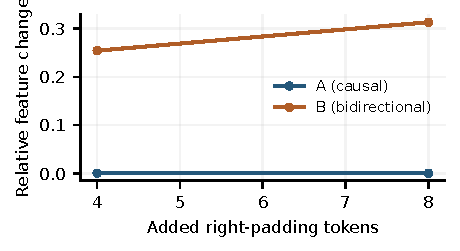
\includegraphics[width=.48\textwidth]{figures/padding_diagnostic.pdf}
\caption{The same random-model implementation check. Competition-score attribution cannot be read
from this curve. The full script and JSON output are included for reproduction.}
\end{figure}

The random-model check establishes a functional sensitivity in the implementation. It does not establish
that 31.3\% is the change in the trained B checkpoint, nor that fixing the mask would recover A's NER
score. Padding is relevant to variable-length padded NER/role/classification batches. Summarization
uses one document per forward and PCR inference groups equal-length chunks, so those paths avoid this
particular source of padding contamination. B's poor retrieval result still needs explanations beyond it.

The stronger global confound is the foundation itself. B has 600 recorded updates versus A's 16,800,
and worse comparable tail loss. Its features come from ten encoder layers rather than A's 22 decoder
layers, while its full parameter count includes a decoder unused in those tasks. A useful next experiment
would first add the missing encoder padding mask, then match training budget or continuation-tail quality,
and only then compare transfer. The report does not assert the outcome of that unperformed experiment.

\section{Concrete generation and retrieval errors}
\label{app:examples}
The summarization notebook prints generated examples as well as scalar scores. In the textile dispute
example, the reference discusses the procedural effect of withdrawing a special-leave petition and the
treatment of the court's order. The generated summary spends its budget repeating wage/dearness-allowance
demands. This is a coverage failure visible in that example, not a quantified dataset-wide factuality rate.
In the 229-word test preview for document 5994, one complete sentence is repeated 17 times. The source and
derived repetition-count audit are retained as metadata without republishing the full raw documents.

Three displayed dev retrieval rankings begin with their own query IDs. For \code{0000035468}, the
dev table records zero hits against 15 positives, and its ranking begins with \code{0000035468}.
That first result is therefore a false positive for this query. The two displayed test examples likewise
begin with their own IDs, but private test labels prevent computing their individual correctness here.
The recorded retriever validates pool membership and uniqueness; it does not exclude query IDs.

Another displayed dev case, \code{0181443842}, has 92 relevant cases and only seven output slots.
Its displayed hit count is three. This yields per-query recall $3/92\approx0.0326$, with a maximum of
$7/92\approx0.0761$ under the required cutoff. The overall metric remains micro-averaged over complete
gold sets, so high-cardinality queries materially affect the denominator.

No specific NER boundary mistake or named rare-role confusion is invented for this appendix. Raw error
examples/confusion matrices for those phases were not saved in the supplied artifacts. The alignment and
role-decoding limitations described elsewhere are implementation facts and hypotheses to investigate.

\section{Configuration provenance, execution and code layout}
\label{app:configs}
The submission has \code{code/phase1/} through \code{code/phase7/}, each with a selected-model source
snapshot, a machine-readable training recipe, a provenance file, a phase README and a command-line
launcher. \code{code/common/} holds shared libraries, all four architecture implementations, adapters,
clean notebooks and tests. Keeping common dependencies separate prevents seven divergent copies of the
same training code. The phase launchers insert that sibling common directory into the Python path.

For phases with no exported winning-run configuration, the recipe is explicitly reconstructed from the
archived source/notebook. The provenance file distinguishes observed fields from defaults and unknown
fields. Such a recipe reproduces the implementation, not necessarily the exact reported score. The
second A rhetorical-role submission is a particular example: its winning settings cannot be inferred
from the later notebook defaults. Recovering its original Drive config would remove that uncertainty.

For later phases, the final saved notebook cell can belong to another model (for example, D's LSI KD
cell). It is not copied blindly as A's exact config. Snapshot metadata, run names, pool/chunk settings and
comparison outputs identify the selected family; unknown A epoch/checkpoint choices remain labelled.
The code supports loading the original run config supplied externally through the launcher.

The intended commands after installing the requirements and obtaining the official data are:
\begin{verbatim}
python code/phase5/run.py train --config code/phase5/recipe.json \
  --phase1-run /path/to/A_qwen_dense_full --data-dir /path/to/p5
python code/phase5/run.py predict --run-dir /path/to/lsi_run
\end{verbatim}
Equivalent launchers cover the other task phases. Phase 1 additionally needs the tokenizer/bin preparation
notebooks. Each phase README describes its required files and output schema. No model weights,
checkpoints, token binaries, HF token, raw dataset or generated prediction dump is included. Environment
authentication supplies dataset access; a token file is not part of the public code tree.

The selected official upload IDs are 965311, 977453, 992390, 1006421, 1016369, 1028885 and 1038509.
Their filenames and four-decimal scores are in the ledger. Local run-to-archive mappings that are inferred
from names rather than settings hashes are labelled accordingly in \code{selected_submission.json}.
The code repository is \url{https://github.com/maheshwari-nitin/cs781}.

\subsection{Checkpoint and interruption behavior}
Phase 1 writes resumable optimizer checkpoints plus best/final weights. Later task loops save their best
inference weights. Several newer loops protect nonempty output folders to prevent accidental overwrites;
they do not implement optimizer resume. Therefore a new run name is required for a fresh fit. A deadline
check happens between optimizer accumulation groups; final dev evaluation and checkpoint writing still
take time after the deadline trigger.

Retrieval batching preserves the selected effective query batch through accumulation. Candidate
sets remain independent within each physical batch, and embedding inference retries the same chunks
with a smaller batch after a failed encoding attempt. These controls change execution batching without
adding in-batch negatives or changing the retrieval objective.

\subsection{Reproduction-sensitive details}
The local summary scorer hash is
\begin{center}\small\code{roberta-large_L17_no-idf_version=0.3.12(hug_trans=5.22.0)}.\end{center}
Its baseline-rescaling/IDF behavior and evaluator model need to match the competition before asserting
identical scores. QLoRA uses bitsandbytes NF4 base projections \cite{bnb}, while C depends on FLA kernels.
Exact historical dependency versions were not fully recorded.

\section{Unexecuted follow-up recipes and negative-mining safeguards}
The longer A retrieval candidate is named \code{A_full__more_steps_v2}. It allows 30 epochs, LR
$3\times10^{-5}$, 3\% warmup, fresh epoch-seeded positive/negative subsamples and six-evaluation patience.
The original context/temperature/effective batch are retained for this candidate. The optional hard-negative
and longer-context candidates change additional factors. They are not listed among measured results.

TF-IDF mining fits only the official TRAIN candidate text, using a sparse word/bigram representation
\cite{sklearn}. All gold positives are excluded from negatives, even when a positive cap means some are
not sampled into the current tuple. A mixture of hard and random negatives avoids training only on one
static lexical neighborhood. Per-epoch tuples and the mined pool are saved. Queries with no lexical
overlap fall back to random sampling. No dev/test relevance enters the training objective.

The A comparison helper checks the Phase-1 weight hash, train/dev fingerprints and actual query subsets.
It chooses from the original measured A run and completed candidates, keeping the original on ties or
regressions. The tuning notebook thus cannot label an unrun candidate as an improvement. Repeated
dev selection still introduces selection bias; the report does not treat its chosen score as an unbiased
generalization estimate.

\section{Verification record and unresolved evidence}
The retained repository regression suite has 13 passing regression tests. It covers multi-label schemas and
calibration, summary masking/shifting and EOT, retrieval pools/metrics, batching-gradient equivalence,
negative exclusion, resampling, early stopping, checkpoint completeness and baseline-preserving selection.
The report's additional padding diagnostic is separately labelled as a new random-model
implementation check.

Before the final PDF was produced, both the notebook format and numerical transcription were checked,
LaTeX was compiled, the ten-page main-body boundary was verified, and the archive was checked for its
two required root directories and absence of weights/credentials. The report package retains sources
so a reviewer can rebuild the PDF and figures. Remaining evidence gaps are exact early winning-run
configs, full Phase-1 corpus/token logs and raw early-phase predictions.
